
\chapter[Mortgage Model]{Mortgage Model}

This appendix contains a fairly complete description of the mortgage model with all the equations and figures.

This model is needed to describe bank/buyer behaviour and to calculate the maximum bid that agents make. Mortgage conditions limit the potential bid.

ADD? the discounting equations for the mortgage period"?
sum\_delta, sum\_r?


\subsubsection{Bank mortgage parameters}

\begin{description}
\item [mortgage period]  mortgage\_period (T)
\item [cost of capital for the bank] r\_prime. The bank's interest rate, $r$, is just the bank rate, (r\_prime) set, for instance, by the Bank of Canada.  
\item [r\_margin] The bank's markup on funds when it lends.  
% \item [r\_target] reference rate that the bank demands on loans on $r^{target}= r^{prime } +r^{margin}$ ? 
\item[lending rate/borrowing rate] The bank lends preferentially to wealthier clients.  
\[r_i=r^{prime} + r^{margin} + \mathrm{individual_wealth_adjustment}\] 

\begin{figure}
    \centering
 \input{fig/price_of_capital}\label{fig-capital-cost}   
    \caption{Individual borrowing rate r\_i}
    \label{fig:Wealth-based}
\end{figure}

 

\item [maximum mortgage share of price] parameter in the calculation of $m_i$. Specific to the functional form used. Set at 0.9. Based on stylized facts from the literature.  No empirical estimates are available. 
\item[wealth sensitivity] of maximum mortgage share of price. This is a parameter in the calculation of $m_i$. It is specific to functional form used. Set at 0.1. The choice of a function is based on stylized facts from the literature.  No empirical estimates are available.  Used in Equation~\ref{eqn-wealth-based-mortgage}.

\item [ability to carry a mortgage] 

The share of income that can be used to cover mortgage interest. (rule of thumb: don't spend more than 25\% or 30\% we use 0.28.)
\end{description}
%

\subsection{Maximum mortgage calculation}
The bank puts two  limits on the size of the mortgage, one based on income and one based on wealth.

% Mortgage gives 2 numbers. First it pays for a share of the purchase price, second it has an actual maximum. 


\begin{figure}
\centering
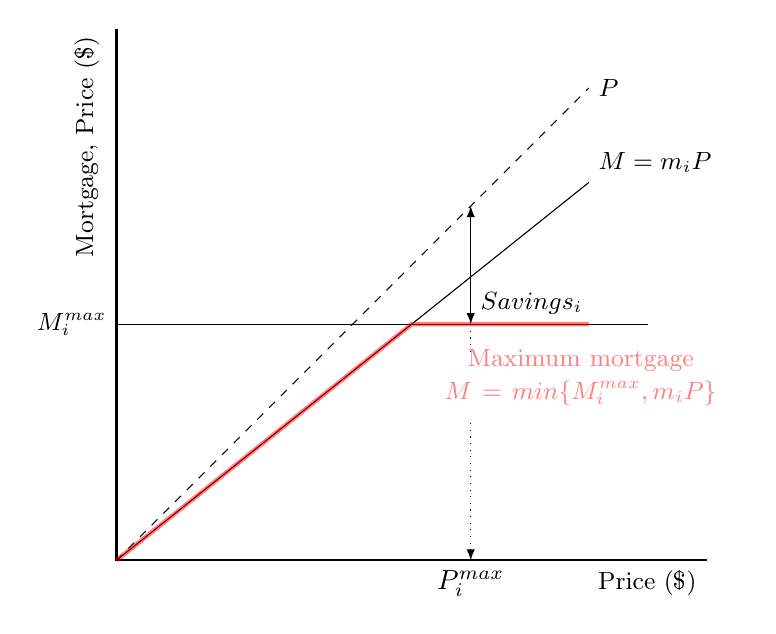
\begin{tikzpicture}	[scale=1.5]
%AXES
\draw[thick] (0,4.5) --(0,0)--(5,0)node[below left]{\small Price (\$)};
\node at (-.25, 3.5)[ rotate=90]{\small Mortgage, Price (\$)};
% M =Mi MAX
\draw[dashed] (0,0)--(4,4)node[right]{\small $P$};
\draw[] (0,2)node[left]{\small $M_i^{max}$}--(4.5,2);%node[right, red]{\small $M = M_i^{max}$};
% M =mi MAX
\draw[] (0,0)--(4,3.2)node[above right]{\small $M = m_iP$};
% COMBINED MAX RED
\draw[ultra thick, red, opacity=.5] (0,0)--(2.5,2)node[below right,  text width=4cm, align = center]{\small \\ Maximum mortgage \\ $M=min\{M_i^{max}, m_iP\}$}--(4.0,2);
% SAVINGS
\draw[latex-latex] (3,2)node[above right] {\small $Savings_i$}--(3,3);
% PMAX
\draw[dotted,latex- ] (3,0)node[below] {$P_i^{max}$}--(3,1.2);
\draw[dotted ] (3,2)--(3,1.72);
\end{tikzpicture}
\caption{The bank's dual mortgage constraint and the savings constraint determine the maximum bid price}
\label{fig:my_label2}
\end{figure}


The two constraints on  mortgage size   that the bank imposes are incorporated in the kinked red line in Figure~\ref{fig:Wealth-based}. The maximum  permitted mortgage  is combined with the savings constraint to determine the maximum price that a potential home buyer can offer.   

% a kink because there are 2 constraints.  The actual mortgage must be below both lines.
The diagonal line, the top dashed diagonal line, is just the price, P = mortgage + savings.
The difference between the two diagonal lines is what the purchaser pays from savings.  
% This is just the constraint. Up to the kink, little $m_i$ is a fraction of price. beyond at little mi becomes a different number - number based on little $m_i$ for everyone
% banks have an advantage since they can practically bid anything
% m - mortgage share
% P - realized price
% M - maximum - 

\begin{figure}
    \centering
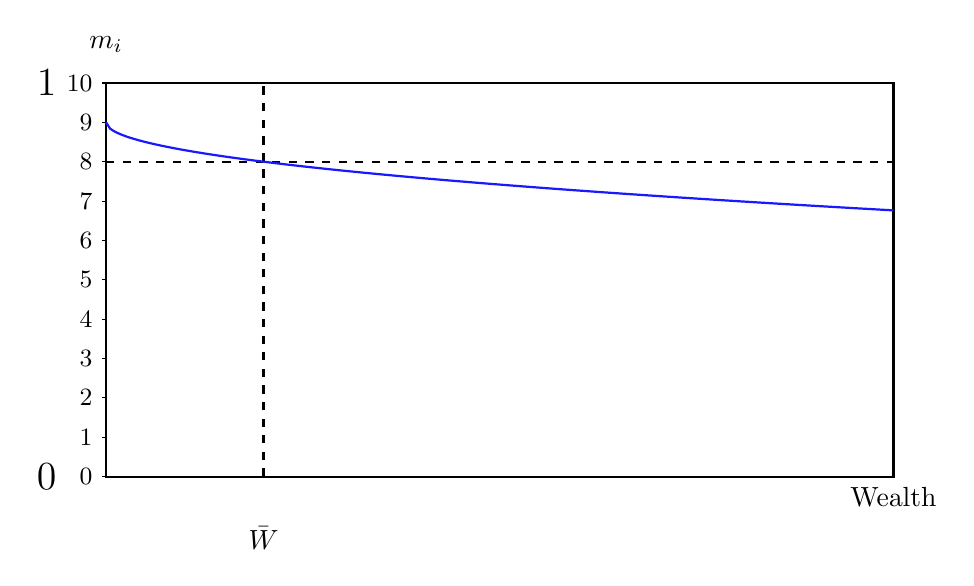
\begin{tikzpicture}[scale=.5]
% \def\bndmax{5}        %https://tex.stackexchange.com/questions/68462/filling-a-complex-region-with-tikz
% \def\bndmin{0.2}
\def\Y{10}  % height of y axis pecent
\def\W{20}  % length  of x axis
\def\Wbar{4}
\def\rbar{8}% this is the prime rate
% Equation   \[ r_i = (A + .5 \frac{\bar{W}}{W_i})\omega\]
% \def\Wmin{.63}  %This sets the lower limit fo the 
\def\Wmin{(\B*\Wbar)/(\Y/\rbar-\A)} %function to keep in in bounds
\tikzset{func/.style={thick,color=blue!90}}	
\draw [thick](\W,\Y)-- (0,\Y)node[left=.5cm]{\Large$1$}node[above=.25cm]{$m_i$} -- (0,0)node[left=.5cm]{\Large$0$}--(\W,0)node[below]{Wealth}--cycle;  	% Axes box
\draw [dashed, thick] (0,\rbar) -- (\W,\rbar);  	% Axes
\draw [thick,dashed] ( \Wbar,0)node[below=.5cm]{$\bar{W}$} -- (\Wbar,\Y);  	% Axes
\foreach \yi in {0,...,\Y} \draw (0,\yi)--(-.1,\yi)node[left]{\small$\yi$};
% \foreach \yi in {0,2,4,6,8,10} \draw (0,\yi)--(-.1,\yi));
% node[left]{\small$\yi$};
% \foreach \yi in {0,2,4,6,8,10}node at (-.1,yi) {{10*yi}} ;
\draw[func,domain=0:\W] plot [samples=200] (\x,(9-\x^.5/2);
\end{tikzpicture}
    \caption{Individual borrowing ratio mi as a function of wealth}
    \label{fig:Individual-borrowing-rate}
\end{figure}


\textbf{Wealth-based mortgage maximum} 
\begin{equation} m_i^{max\_permitted} = 0.9-\left(\frac{W_i}{\bar W}\right)^{0.1} \end{equation} \label{eqn-wealth-based-mortgage}

% **Source**: Ch:model line 580, page 87.. I have done some fiddling Wealth $W_i = P-M+S.  for i - real estate agents estimated price wealth of a property owner as assessed by the bank.

Where 0.9 is the maximum fraction that can be mortgaged and 0.1 is the wealth sensitivity parameter.


\textbf{Income-based  mortgage maximum}

\[M^{max\_permitted}_i\ = \frac{0.28*(\omega+\psi+ r_{prime}* \mathrm{savings})}{r_i}\]
Where 0.28 is a parameter for \gls{ability to cover a mortgage}, the maximum the bank will let an applicant pay based on their wealth.
 
\textbf{Combined  mortgage maximum}

The above  two equations specify two constraints on the mortgage,  combining we get:
\begin{align} 
M_i^{max} &= min \left\{ m_i^{max\_permitted}*P, \ M^{max\_permitted}_i \right\} \\
&= min \left\{ \left(0.9- \left( \frac{W_i}{\bar W}\right)^{0.1}\right)P, \  \frac{0.28*(\omega+\psi)}{r_i} \right\} 
\label{eqn-max-mortgage2}
\end{align}

\begin{lstlisting}


get_max_bid

\end{lstlisting}

We assume that a buyer always takes the maximum mortgage available. Doing so maximizes the financial return on the transaction. % That means that the  


\subsubsection{maximum price that one can bid} is $ P_i^{max}=M_i^{max} + \mathrm{savings_i}$.


\subsection{Maximum bid}
The maximum price a person can bid is 

\begin{align}
P_i^{max\ bid}= min \left\{\frac{\mathrm{savings}_i}{1-m_i^{max\_permitted}},\ \mathrm{saving}s_i + M_i^{max\_permitted}  \right\}     
\end{align}
 
where little $m_i$ is a ratio, capital $M_i$ is a dollar value


\subsubsection{Bid price for first-time buyer}
Use $P_i^{max}$  as we used to call ``maximum bid'' in the bargaining process.
 

\subsubsection{reservation price}
Sellers should use the calculated before  as their reservation price in the bargaining process. If they can't get a higher price they  can keep the home as a rental  investment and use the home as collateral for a mortgage on a house in the country.

\subsubsection{Bid price for second home buyer}
A second home buyer may have a mortgage. The bank will require that the sum of the two mortgages be supportable. 




\subsection{Maximum bids}
The maximum price in Equation~\ref{eqn-property-investment-return1} that the investor can price offer for the property  and still satisfy the inequality~\ref{eqn-property-investment-return2} $P_B^{max}$ is



TODO: Need to consider the case where it is better to rent/not-buy. Need the market rent for every house. What would you rent it out for.
\begin{eqnarray}
P_{person}^{max\_bid} & = min \left\{\frac{\mathrm{savings}_i}{1-m_i^{max\_permitted}},\ \mathrm{saving}s_i + M_i^{max\_permitted}  \right\}  \label{eqn-bid-price-P} \end{eqnarray}


\begin{eqnarray}
P_{bank}^{max\_bid} & =   \frac{\mathcal{R}_N}{(1-m)r^{target}-\delta \left(1 + \dot P_M^e - (1+r)m\right)} \label{eqn-bid-price-B} \end{eqnarray}

\subsection{Reservation prices}

For a homeowner, the reservation price is tricky. 
At this point we only have retirement as a hard boundary to consider. We assume that a homeowner can move to the country and purchase a home for $\frac{a\psi}{r_prime}$. Since at the moment there are no urban amenities and no transaction costs, the gain from moving to the country is \begin{equation}
P_{ij}^{expected}-\frac{a\psi}{r_prime}    
\end{equation}\label{eq:movers-gain}

This amount is added to savings in retirement, increasing consumption. 
We could subtract an urban amenity term, $U_{ij}$ and an transaction cost from equation~\ref{eq:move3rs-gain}. The amenity term is likely to have little effect, since a buyer will pay extra for the amenity. 

My suggestion is that $P_{ij}^{expected}$ is the \textbf{initial reservation price}. If the seller does not get this  she reduces the reservation price for the next period by (say) 5\% .

\subsubsection{expected price}
So what is the \textbf{expected price}? this should be the expected price from a weighted price regression.\footnote{Wheaton \cite{wheatonVacancySearchPrices1990} suggests ``The combination of price and expected sales time determines the ``expected price'' for a house: market price discounted by expected sales time.'' In his model, vacancy, matching, sales time, and prices with positive vacancy, matching, sales time, and prices are all jointly determined.} Crudely it might be
\[P_{d,t}^e=\beta_1 d + \beta_2 P_{d,t-1} +\epsilon\]
where $\beta_1$ captures spatial correlation and $\beta_2$ captures serial correlation. In this model $\beta_2=1+\dot P$. This simple relationship would tend to change in each period, so the regression would be repeated  at the end of each period  to be used by everyone in the next period. 

You could add $+ \beta_3 (P_{d,t-1}-P_{d,t-2})$ to capture the changing  price change. 

\textbf{Alternative approaches to the reservation price}

\begin{eqnarray}
P_{person}^{reservation} & =   \frac{\mathcal{R}_N}{(1-m)r^{target}-\delta \left(1 + \dot P_M^e - (1+r)m\right)} \label{eqn-res-price-P} \end{eqnarray}
For the bank the problem is easier = if an9yon offers more that the maximum bid, the bank should sell
\begin{eqnarray}
P_{bank}^{reservation} & =    \frac{\mathcal{R}_N}{(1-m)r^{target}-\delta \left(1 + \dot P_M^e - (1+r)m\right)} \label{eqn-res-price-B} \end{eqnarray}

% P_B & \le    \frac{\mathcal{R}_N}{(1-m)r^{target}-\left[ \delta(1+L(P)- (1+r)m\right]}
We call this  $i's$ maximum bid and compute it for all potential buyers and sellers. In each sale the highest $P_B$ will make the purchase. The denominator can be seen as an adjusted rate of return for capitalizing net rents, analogous to the value of $r$ in  the standard capitalization formula. 


% \begin{tabular}{p{1.5cm}|p{4.5cm}|p{4.5cm}}
%     & reservation & maximum bid\\\hline
% person-buyer    &   & $min \left\{\frac{\mathrm{savings}_i}{1-m_i^{max\_permitted}},\ \mathrm{saving}s_i + M_i^{max\_permitted}  \right\} $ \\\hline
%    person-new  &   & $min \left\{\frac{\mathrm{savings}_i}{1-m_i^{max\_permitted}},\ \mathrm{saving}s_i + M_i^{max\_permitted}  \right\} $ \\\hline
% Bank    &$ min \left\{\frac{\mathrm{savings}_i}{1-m_i^{max\_permitted}},$$\newline$$\mathrm{saving}s_i + M_i^{max\_permitted}  \right\}  $ & \hline
% \end{tabular}

% ALTERNATIVE, NOT USED CALCULATION
%An alternative way to do this, based on old calculations is to compute the realized mortgage share. The realized mortgage $m_i$

%$m_i$ is follows the wealth based rule, $m_i*$ follows the savings based mortgage rule. The realized mortgage share is whichever of these is chosen by the rule in Equation~\ref{eqn-max-mortgage}.

%$m_i^*$, and get the savings.
% We use $m_i$ in calculating the maximum bid for individuals.
%The \textbf{maximum bid} (price that will be offered) is the minimum of $M^{max_i} +S$ and the maximum bid calculated using $m_i$, , (which is calculated independently) if price
% $P\le \frac{M_i^{max}}{m_i}$ 
% and $m_i^*$ if 
% $P\ge \frac{M_i^{max}}{m_i}$, where 
% \[m_i^*=\frac{M_i^{max}}{P}\]

\subsection{Price setting}
\textbf{We have a many-to-many matching problem}. Many buyers and sellers single sellers for each unit. Therefore, for each property that comes on the market each potential seller has a reservation price $P_{ij}^{reservation}$ and there will be a set\footnote{We could allow potential buyers  to approach potential sellers who have not listed with an offer and allow worker-owners to consider retiring early or becoming tenants if an offer is attractive.  This is only likely if speculative pressures are strong. It may require having multiple institutional buyers to make offers more competitive. In that case, initial offers will be closer to the maximum bid price, tending to pull prices up and benefit potential sellers.}  of potential buyers with maximum bids $P_{ij}^{maxbid}$.


This will appear in your data as a set of bids and a reservation price for each property on the market that must be converted to a price for that property using the bargaining rule. The rule is simple: 
\begin{enumerate}
    \item if there is only one maximum bid above the reservation price, split the difference.

    \item If there are two or more maximum bids above the reservation price, the property goes to the highest  and the price is the second highest
\end{enumerate}

\subsubsection{The process}
\begin{enumerate}
\item \textbf{identify the pool of sellers} for each cycle.
    \begin{enumerate}
        \item Agents who a) own and b) age out
        \item Agent  who failed to sell in the previous period.
        \item the bank
    \end{enumerate}
\item \textbf{identify the pool of buyers} 
    \begin{enumerate}
        \item the bank. May buy many, (There must be a capital (C) constraint something like $C/\bar P$ to select a number of bank bids in any period.)
     \item newcomers, 
     \item individuals as investors.
     \item the bank
    \end{enumerate}

\item \textbf{count buyers and sellers} and use the counts to identify sellers or buyers' market. \# Sellers > \# buyers is a buyers/ market. For a buyer's market  choose the lower price. \footnote{.The is often done with buyers/vacancies. Changes in this ratio are observed to trigger significant movement in rent r market prices.\cite{wheatonVacancySearchPrices1990}. Lisi and Iacobini \cite{lisiEstimatingHousingPrice2015} found  that in the Italian market, ``the difference between the actual selling price and the price obtained in an ideal situation of frictionless housing market – is remarkable. ... the higher the trading frictions on the demand side (more buyers and less sellers), the higher the actual selling price (the price adjustment is positive), whereas the higher the trading frictions on the supply side (less buyers and more sellers), the lower the actual selling price (the price adjustment is negative). '' (they point out that ``Trading frictions are obvious in the housing market, as it takes weeks or months to buy or sell a house (Caplin and Leahy, 2011; Rocheteau and Weill, 2011).'')}  

%a key role is played by the so-called “time-on-the-market (TOM)”. The time it takes to sell a property or “the expected time until the asset is sold when following the optimal policy” (Lippman and McCall, 1986) – commonly known as the TOM – measures the degree of illiquidity of the real estate asset and is a fundamental characteristic differentiating real estate from financial assets. \cite{lisiSearchMatchingProcess2019}
\item \textbf{The pooling problem}  Houses should go at different prices if they have different net rents.  Assume buyers and sellers are indifferent about location (no  local amenities) so only the net rent matters for the ban and only the full rent for individuals.

\item \textbf{Create lists} for the buyer pool and the seller pool. (The bank can appear on the list many times.) 

If the market is efficient, the allocation will maximize the sum or seller and buyer surplus.

\item To select the set of transactors, \textbf{order the lists}. Buyers from highest to lowest, sellers from lowest to highest.

\end{enumerate}


that they are of the same length by dropping the lowest bids or the highest reservation prices. 

\newpage
\textbf{Possibly relevant Example of a matching problem drawn from my game theory text}

There are 26  people, some with houses, Each values the house an amount equal to the last three digits of their student numbers. Those on the left of the table don't have a house when the game starts, indicated by a ``0'' in the second column. Those on the right  start with a horse, indicated by a  (1) in the fifth column and half don't. 

\begin{center}
Value and number of houses

\begin{tabular}{|c|c|}
 
\begin{tabular}{lcc}
max bid&start&end  \\ \hline
985  & 0 & 2 \\
829  & 0 & 1 \\
740  & 0 & 1 \\
650  & 0 & 1 \\
643  & 0 & 1 \\
611  & 0 & 1 \\\hline
532  & 0 & \color{red}1  \\
356  & 0 & \color{red} 1   \\
270  & 0 & \color{red} 1  \\
135  & 0 & 0    \\%69 & 1  & 0
   
\end{tabular}

&
\begin{tabular}{lcc}
reservation&start&end \\ \hline
 50 & 1  & 0 \\
127 & 1  & 0 \\
190 & 1  & 0  \\
245 & 1  & 0 \\
 324 & 1  & 0 \\
 522 & 1 & \color{red} 1\\\hline
 738 & 1  &  \color{blue}0 \\
 829 &1  &  \color{blue}0 \\
832 & 1 & \color{blue}0\\
   &  &              \\%69 & 1  & 0 
\end{tabular}

\end{tabular}
\end{center}


 
  \begin{tikzpicture}[scale=.8]
%  \draw [gray, opacity=.7]
 (0,0) grid (7,7);
\draw [<->] (0,10.5) node[above]{value}-- (0,0) -- (10,0) node[below]{Houses};

\draw [red, thick] (0,9.85)node[above right]{985}--(1,9.85)--(1,8.29 )node[above right]{829}--(2,8.29 )--(2,7.40 )node[above right]{740}--(3,7.40 )--(3,6.50 )node[above right]{350}--(4,6.50 )--(4,6.43)node[above right]{643}--(5,6.43)--(5,6.11)node[above right]{611}--(6,6.11)--(6,5.32)node[above right]{532}--(7,5.32)--(7,3.56)node[above right]{356}--(8,3.56)--(8,2.70)node[above right]{270}--(9,2.70)--(9,1.35)node[left]{DEMAND}node[above right]{135}--(10,1.35); 

\draw [blue, thick] (0,.50)node[above right]{50}--(1,.5)--(1,1.27 )node[above right]{127}--(2,1.27 )--(2,1.90 )node[above right]{190}--(3,1.90 )--(3,2.45 )node[above right]{245}--(4,2.45 )--(4,3.24)node[above right]{324}--(5,3.24)--(5,5.22)node[above right]{522}--(6,5.22)--(6,7.38)node[above right]{738}--(7,7.38)--(7,8.29)node[above right]{829}--(8,8.29)--(8,8.32)node[above right]{832}--(9,8.32)node[right]{SUPPLY}; 
%,2.5) ;
%\draw [blue, dashed] (0,4.5) node[left]{large bill}--(8.33, 4.5)-- (8.33,0)node[below] {large user Q};
%\draw [green, dashed] (0,0) --(8.33, 4.5);
%\draw [green, dashed] (0,0) --(1.66, 2.5);

%\draw [<->, shift={(7 cm,0)}] (0,6) -- (0,0) -- (5,0);
\end {tikzpicture}

The gain for any person is the difference between the transaction price  for a house and the amount they value a house




At the same time, for each p. NOT. DONE
\begin{eqnarray}
P_{bank}^{reservation} & \le  P_{person}^{max\_bid} \end{eqnarray}


\begin{lstlisting}
# parameters - max interest payment 
max_mortgage_share = 0.28 # ability to cover a mortgage

# Max mortgage

wealth = property_value - mortgage + savings
mean_weath = sum(wealth)/number_of_people

def get_max_mortgage(self, applicant):
    max_mortgage =  ...
    
    return max_mortgage
\end{lstlisting}


